%% SW arkitektur: Data View

I forbindelse med EasyWater8000s log skal der gemmes data på en nem og håndterbar måde. Det skal være muligt at gemme følgende data:

\begin{enumerate}
	\item Tidsstempel
	\item Temperatur
	\item Fugtighed
	\item Bevægelse
	\item Vanding
\end{enumerate}

Ydermere skal disse informationer gemmes for hver enhed. Så hvis der er 18 huller med i alt 18 enheder, skal ovenstående gemmes for alle 18 enheder.

Når informationen skal præsenteres for brugeren skal det ske i en tabel som vist på figur \ref{fig:GUI-log-alle} i afsnit \ref{subsec:GUI}, data for en enkelt enhed som på figur \ref{fig:GUI-log-enhed} i afsnit \ref{subsec:GUI} eller på en graf så man kan se ændringer over tid som vist på figur \ref{fig:log-graf}.

\begin{figure}[htbp] \centering
{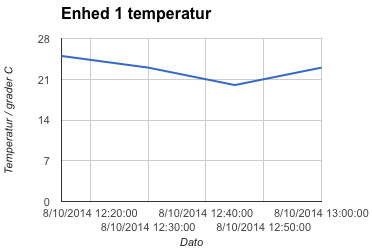
\includegraphics[scale=0.5]{filer/pics/SW-Log-graf}}
\caption{Graf for temperatur for én enhed}
\label{fig:log-graf}
\end{figure}

Tabellen skal have en fane for hver opkoblet enhed. Her kan man se informationer fra hver enkelt enhed. Det bør også være muligt at se alle enheders informationer samtidigt.

Dataen struktureres i semikolon-separerede filer (\verb+.csv+) på Master. Hver enhed har en fil hvor alle data er samlet med udgangspunkt i strukturen vist i liste \ref{list:log-csv-struktur}.

\begin{lstlisting}[caption=Semikolon-separeret datafil til log af enheder, label={list:log-csv-struktur}]
<enheds-nr>;
<KP-nr>; <dato>; <temperatur>; <fugtighed>; <bevaeglse>; <vanding>;
<KP-nr>; <dato>; <temperatur>; <fugtighed>; <bevaeglse>; <vanding>;
...
<KP-nr>; <dato>; <temperatur>; <fugtighed>; <bevaeglse>; <vanding>;
\end{lstlisting}

Dette resulterer i en filstruktur som vist på liste \ref{list:log-fil-struktur} hvis der er koblet 18 enheder op på Master.

\begin{lstlisting}[caption=Filstruktur for logfiler på Master, label={list:log-fil-struktur}]
<log>/
  <enheds-nr1>.csv
  <enheds-nr2>.csv
  ...
  <enheds-nr17>.csv
  <enheds-nr18>.csv
\end{lstlisting}

Hyppigheden for målingerne og logningen er beskrevet i de ikke-funktionelle krav, \ref{header:ikke-funk}.
